%----------------------------------------------------------------------------------------
%----------------------------------------------------------------------------------------
%----------------------------------------------------------------------------------------
%Results
%----------------------------------------------------------------------------------------
%----------------------------------------------------------------------------------------
%----------------------------------------------------------------------------------------
\section{RESULTS and DISCUSSION}
\label{sec: result}
    In this section we are showing the results of trained neural networks, using K96 data. 
    To have a realistic model of the input data we created SOMs with various sizes in both 1D and 2D.
    We start our analysing by creating 1D SOMs. 
    First, we created SOMs with only two neurons (1$\times$2 map) and then we increased number of neurons one at a time in 1D case (~\ref{sec: 1D}).
    Then we generated 2D networks (~\ref{sec: 2D}), and once again we start with smallest number of neuron possible (4 neurons in 2$\times$2 map) and then increased the number of neurons to 144 in 12$\times$12 map.
    
    For each generated network, we compare the results with K96 categorization.
    We also used these networks to classify the T12 galaxies samples, and compare them with classifications from supervised network.
    \subsection{1D SOMs}
    \label{sec: 1D}
        \subsubsection{TRAINING THE NETWORKS}
        \label{sec: 1Dt}
            We assumed that galaxies can be divided only in two types; quiescent and star burst, and then generated a network with only two neurons.
            Then we increased size of the maps gradually till we separated the input 12 sample galaxies into the 12 neurons. 
        
            Figs.~\ref{fig: 1by2T} -~\ref{fig: 1by3T} show results of training network.
            Upper part of the figures shows neurons and their relative distances ($D_j$) from each other.
            As it was mentioned in the Sec.~\ref{sec: method}, the colours between neurons represents the relative distance $D_j$ between the neurons and the darker is the colour the more $D_j$ is between them.
            The lower part shows how many galaxies from K96 template places in each neurons. 
        
        
            In upper side of the Fig.~\ref{fig: 1by2T}, the red colour between two neurons indicate that the $D_j$ between these two groups are relatively high, and these two groups are distinguishable groups.
            In the lower part of the Fig.~\ref{fig: 1by2T}, we see galaxies divided to two groups of 5 and 7.
            Although we know from K96 and T12 that 6 of the galaxies are quiescent and the other 6 are star bursts, the SOM results show 5 of the galaxies in one group and the other 7 in the second group.
            In this method, the Sc galaxies have been categorized as star burst galaxy due to their high amount of the emission lines.
        
            %add more about why Sc is acting differently
            %\import{~/images/texes/}{1by2_t.tex}
            \begin{figure}
                \begin{subfigure}[b]{0.5\textwidth}
                    \centering
                    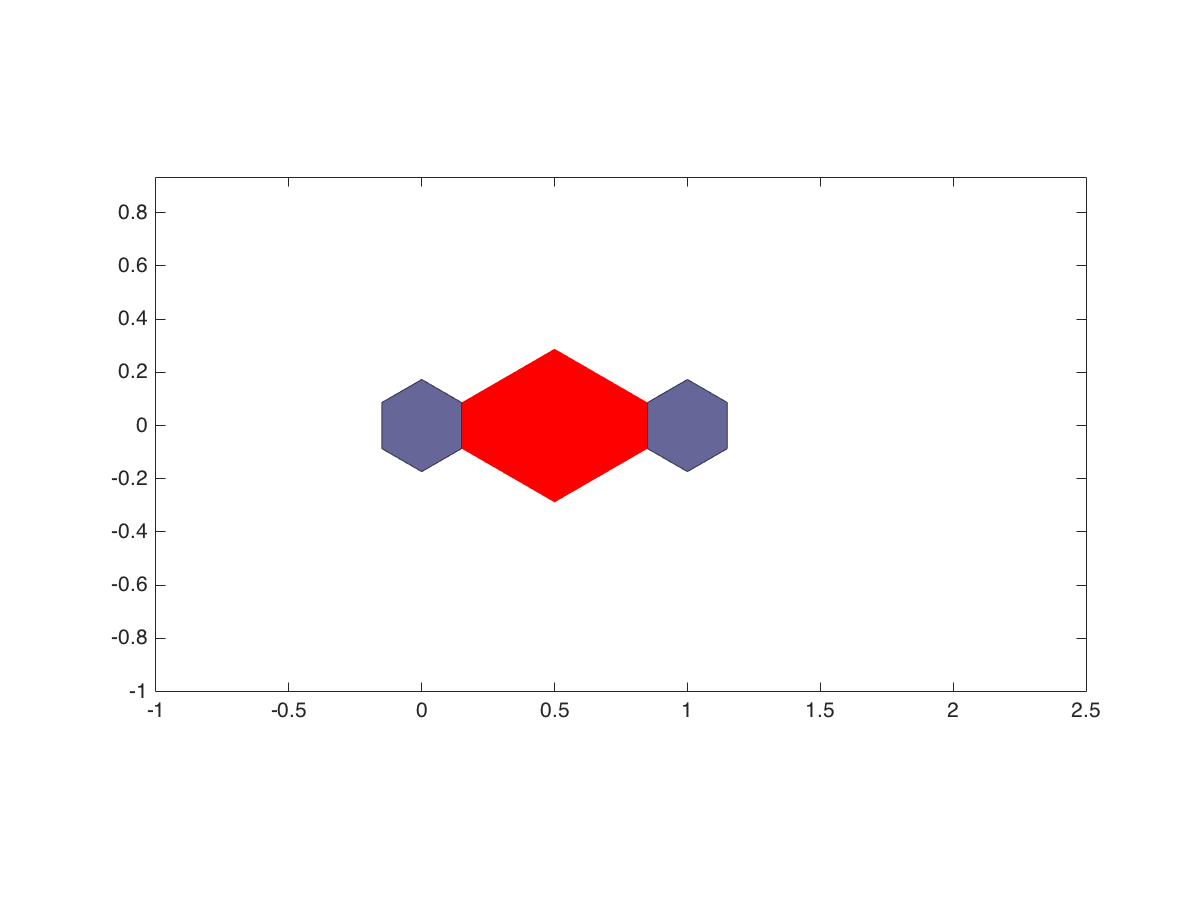
\includegraphics[width=\textwidth]{../images/1d/dist_1_by_2.png}
                    %\caption{$1\times2$ weight map}
                     %\label{fig: 1by2T}
                \end{subfigure}
                \hfill
                \begin{subfigure}[b]{0.5\textwidth}
                     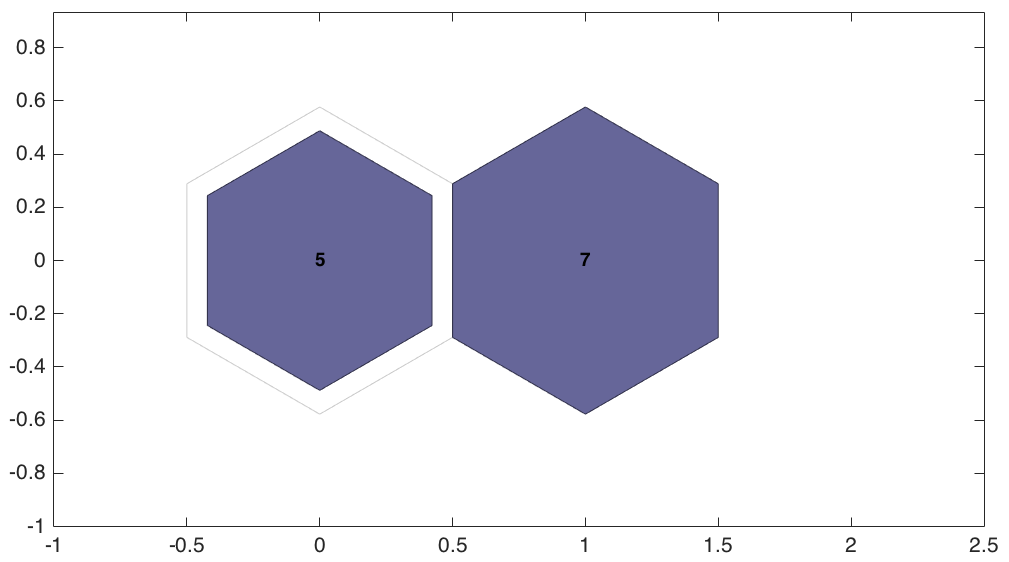
\includegraphics[width=\textwidth]{../images/1d/hit_t_1_by_2.png}
                     %\caption{$1\times2$ hits map}
                     %\label{fig: 1by2Thits}
                \end{subfigure}
                \caption{Results of training network in $1\times2$~grid. In this network, 5 of galaxies from K96 model, categorized as quiescent galaxies and the rest are star bursts. Because of their high emission lines, Sc galaxies moved towards the star burst ones.}
                 \label{fig: 1by2T}
            \end{figure}
        
            Fig.~\ref{fig: 1by3T} shows results of the training in a 1$\times$3 network.
            In these plots we forced the galaxies to categorized themselves in maximum 3 groups. 
            If the galaxies in Fig.~\ref{fig: 1by2T} are very similar to each other or are exactly the same, they still want to be divided in two groups and left the middle node empty. 
            However, in the lower part of the Fig.~\ref{fig: 1by3T}, we can see that the middle node contains two galaxies.
            These two galaxies, which are separated from group of star bust galaxies in the lower part of Fig.~\ref{fig: 1by2T},are types SB5 and SB6 galaxies.
            In upper plot of the Fig.~\ref{fig: 1by3T}, the colour between two right neurons is black and the colour between two left neurons is yellow. 
            The black colours indicates that the left neuron is completely different from the other two groups, while the yellow colour shows the two neurons are very similar to one another. 
            
            Comparing Fig.~\ref{fig: 1by2T} with Fig.~\ref{fig: 1by3T} shows us that the star burst galaxies are divided to two groups. 
            Based on the colours between these two groups, we conclude that they are very similar groups; both groups are star burst galaxies and have strong emission lines.
            However, these two groups have the most internal colour extinctions, so they intend to move more towards the early type galaxies.
                
            \begin{figure}
                \begin{subfigure}[b]{0.5\textwidth}
                    \centering
                    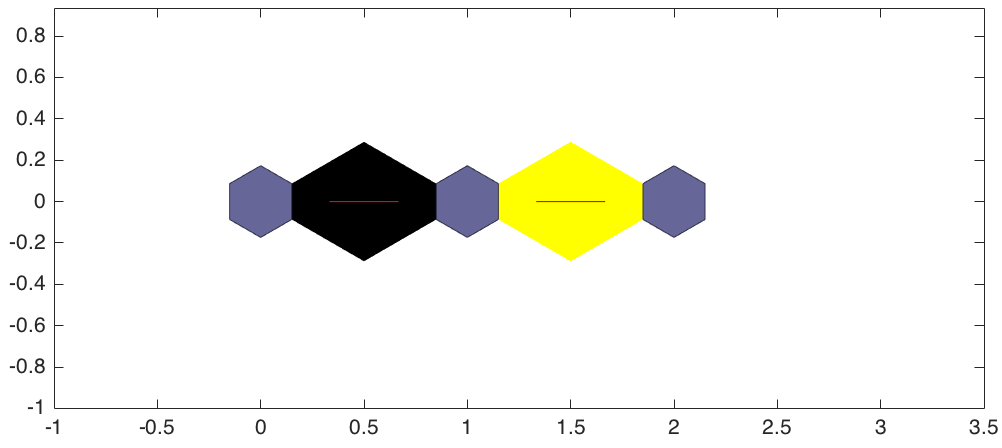
\includegraphics[width=\textwidth]{../images/1d/dist_1_by_3.png}
                    %\caption{$1\times2$ weight map}
                     %\label{fig: 1by3T}
                \end{subfigure}
                \hfill
                \begin{subfigure}[b]{0.5\textwidth}
                     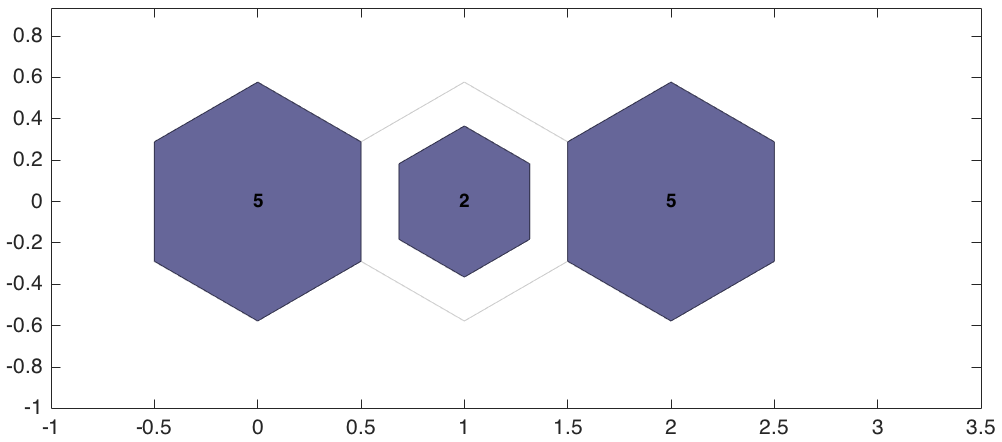
\includegraphics[width=\textwidth]{../images/1d/hit_t_1_by_3.png}
                     %\caption{$1\times2$ hits map}
                     %\label{fig: 1by3Thits}
                \end{subfigure}
                \caption{Results of training network in $1\times3$~grid. In this network again, 5 of galaxies from K96 model, categorized as quiescent galaxies, and 7 as star bursts. However, this time 2 of galaxies (SB5, and SB6) are separated star bursts groups.}
                 \label{fig: 1by3T}
            \end{figure}
           
            We increased the size of maps gradually till the galaxies were divided into twelve groups (Figs.~\ref{fig: 1by4T} to ~\ref{fig: 1by20T} and ~\ref{fig: 1by22T}).
            Since there are more nodes when with increasing the size of map, program pays more attention to small differences between each groups.
            Higher the size of the maps means that even considering the smallest differences between galaxies.
            If the galaxies from K96 had completely different and distinct SED, SOM with size of $1\times12$ were expected to show 12 different groups of galaxies (1 each node).
            However, in Fig.~\ref{fig: 1by12T}, we see that three of neurons contains two galaxies and  three of them are empty. 
            In Fig.~\ref{fig: 1by12T} from left to right galaxies with types of B and E, SB3 and SB4, and SB1 and SB2, are the ones groups together, respectively. 
            The SB3 and SB4 grouping breaks when we increased the size of the map to $1\times15$~(Fig.~\ref{fig: 1by15T}).
            The SB1 and SB2 galaxies remained in the same neurons till we increased the size of map to $1\times20$~(Fig.~\ref{fig: 1by20T}), and the separation between galaxies B and E does not happened before the size of the SOM reached to $1\times22$~(Fig.~\ref{fig: 1by22T}).
        \begin{figure*}
            \begin{subfigure}[b]{\textwidth}
                \centering
                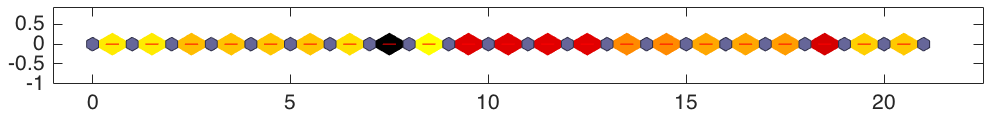
\includegraphics[width=\textwidth]{../images/1d/apps/dist_1_by_22.png}
            %\caption{$1\times22$ weight map}
             %\label{fig: 1by22T}
            \end{subfigure}
            \hfill
            \begin{subfigure}[b]{\textwidth}
                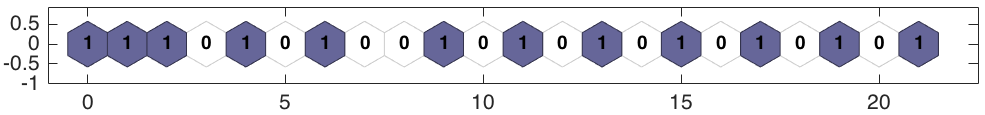
\includegraphics[width=\textwidth]{../images/1d/apps/hit_t_1_by_22.png}
             %\caption{$1\times22$ hits map}
             %\label{fig: 1by22Thits}
            \end{subfigure}
            \caption{Results of training network in $1\times22$~grid.}
            \label{fig: 1by22T}
        \end{figure*}
    
            In Fig.~\ref{fig: 1by22T}, although in lower plot we can see twelve different groups, but in upper plot 5 groups are in the left side neurons and there is a black colour between them and then the rest of the galaxies. 
            It shows that although we separated the galaxies in twelve groups but they are still divided by two main groups.
            The closest occupied neurons in the star burst side of the SOM, belongs to the SB6 type. 
            This type of the galaxies have the most extinction and its SED has similarity to early type galaxies more than other star burst types. 
            
            The fact that the galaxies had to have 22 different neurons till be divided to 12 groups, shows that the difference between SB1 and SB2, and B and E galaxies are very small.
            These small differences might be very hard to distinguish in normal classification methods and might lead to wrong classifications.

        \subsubsection{ CLASSIFYING SAMPLE OF GALAXIES}
            We used each network that we trained in Sec.~\ref{sec: 1Dt}, to classifying the sample 142 galaxies from T12.
            Upper plot in the Fig.~\ref{fig: 1by2V} shows the result of the classifying of the T12 galaxies using the $1 \times 2$~network from Fig.~\ref{fig: 1by2T}.
            It shows that 80 of the galaxies have SEDs similar to the early type galaxies and the SEDs of the rest of them are similar to star burst galaxies.
            The lower plot shows the average SED of the SEDs galaxies in each node. 
            The left plot shows the average SED of 80 galaxies that classify as an early type galaxies. 
            These are the similar ones sit on the left node in the upper plot in the Fig.~\ref{fig: 1by2T}.
            The plots clearly shows the 4000\AA~break in the SEDs, which is the one of the signatures of the SED of the early type galaxies.
            The strong the emission line in that figure comes from the galaxies with similar SED to Sa galaxies but with more strong emission lines.
            The right plot in the lower part of the Fig.~\ref{fig: 1by2V} shows strong emission lines and high emissions in the lower wavelengths, which are the signs of the strong star formation in the galaxies. 
            \begin{figure}
                \begin{subfigure}[b]{0.5\textwidth}
                    \centering
                    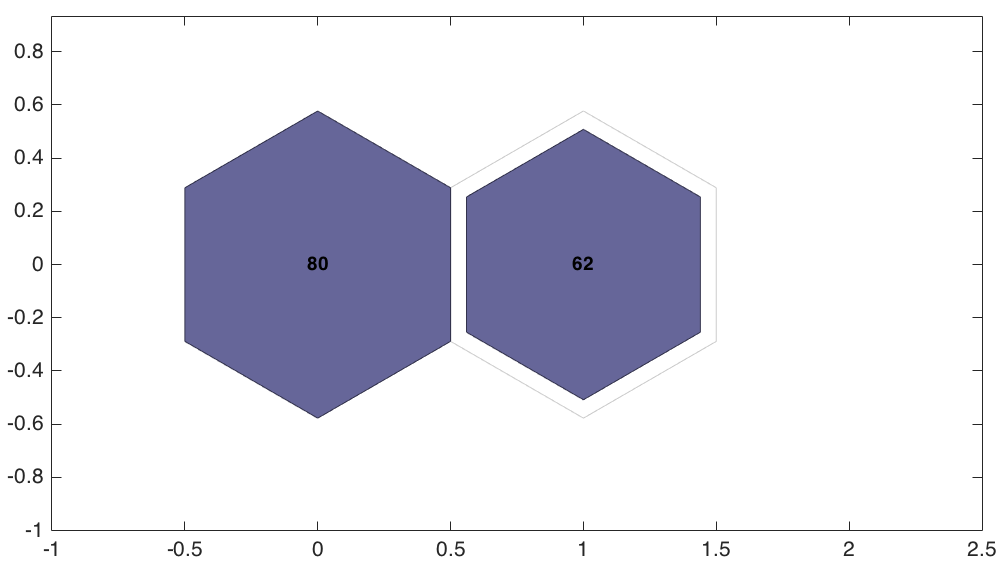
\includegraphics[width=\textwidth]{../images/1d/hit_v_1_by_2.png}
                    %\caption{$1\times2$ weight map}
                     %\label{fig: 1by3T}
                \end{subfigure}
                \hfill
                \begin{subfigure}[b]{0.55\textwidth}
                     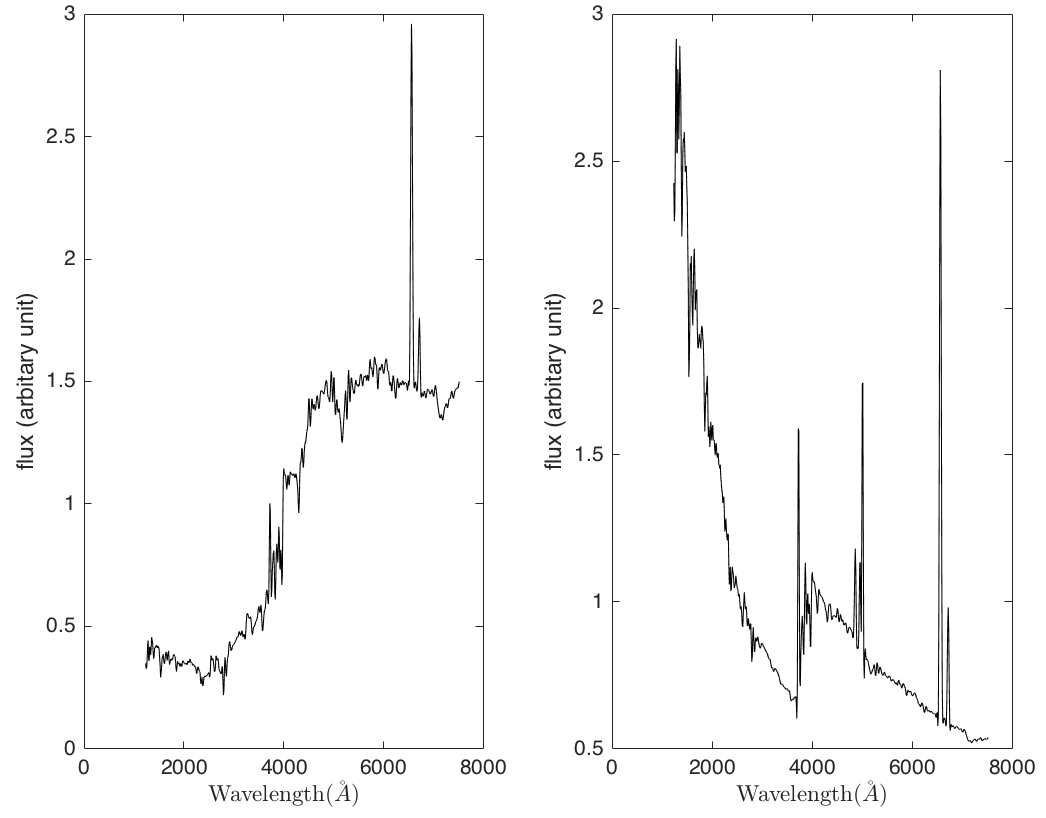
\includegraphics[width=\textwidth]{../images/1d/SED_total1by2.png}
                     %\caption{$1\times2$ hits map}
                     %\label{fig: 1by3Thits}
                \end{subfigure}
                \caption{Classifying galaxies from T12, based on their SEDs using $1\times2$~networks that were trained from 12 galaxies from K96. Up: Numbers in each node represents the number of galaxies that belong to that group. In this case 80 means that 80 of the 142 galaxies classify as the early type groups while the 62 of the 142 galaxies categorize to the star burst galaxies. Down: Average SED of the SEDs of the galaxies in each group. the left plot shows the average SED of the 80 galaxies (early type ones), and the right plot shows the average SED of the SEDs of 62 galaxies (star burst ones).}
                \label{fig: 1by2V}
            \end{figure}            
            Since in this network galaxies forced to divided to two groups, for any SED between these two groups the SOM decides that the galaxy belongs to which group based on the strongest features of its SED.
            The galaxies with a weak 4000\AA~break but strong emission lines and increase of the flux in the lower wavelengths categorized as star bursts while galaxies with strong 4000\AA~break, but high emission lines categorized as the early type.
            Increasing the size of the SOM helps to solve problem of the galaxies which have features of both groups.
            
             Fig.~\ref{fig: 1by3V} represents the result of the classifying the SED of the galaxies using the $1\times3$~network ( Fig.~\ref{fig: 1by2T}). 
             In the upper plot of this figure we can see 66 of the galaxies belongs to the early type group, and 47 belong to star burst galaxies. 
             29 of the galaxies are more similar to star burst ones but, not with all of their features. 
             These group of galaxies have strong emission lines and the ascending slop towards the lower wavelengths, but they also have a strong 4000\AA~break, which makes them to move towards the early type galaxies (middle plot in the lower part of the Fig.~\ref{fig: 1by2V}).

            \begin{figure}
                \begin{subfigure}[b]{0.5\textwidth}
                    \centering
                    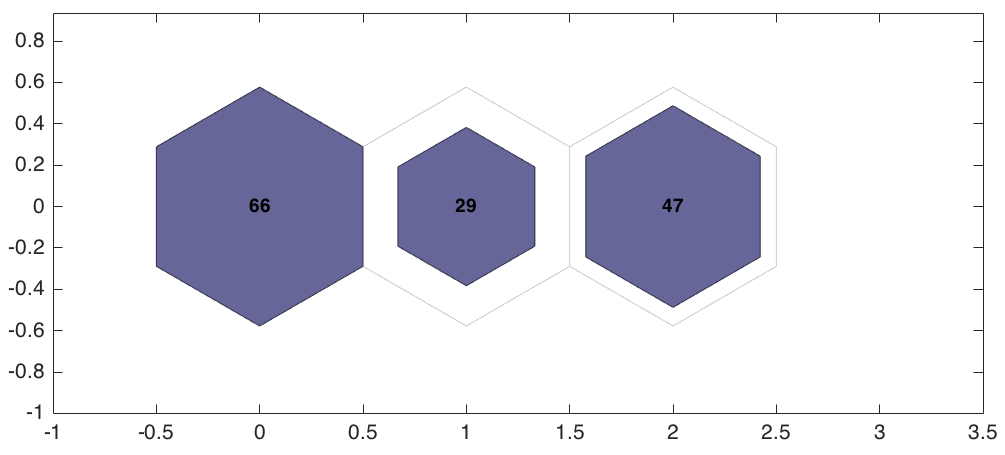
\includegraphics[width=\textwidth]{../images/1d/hit_v_1_by_3.png}
                    %\caption{$1\times2$ weight map}
                     %\label{fig: 1by3T}
                \end{subfigure}
                \hfill
                \begin{subfigure}[b]{0.55\textwidth}
                     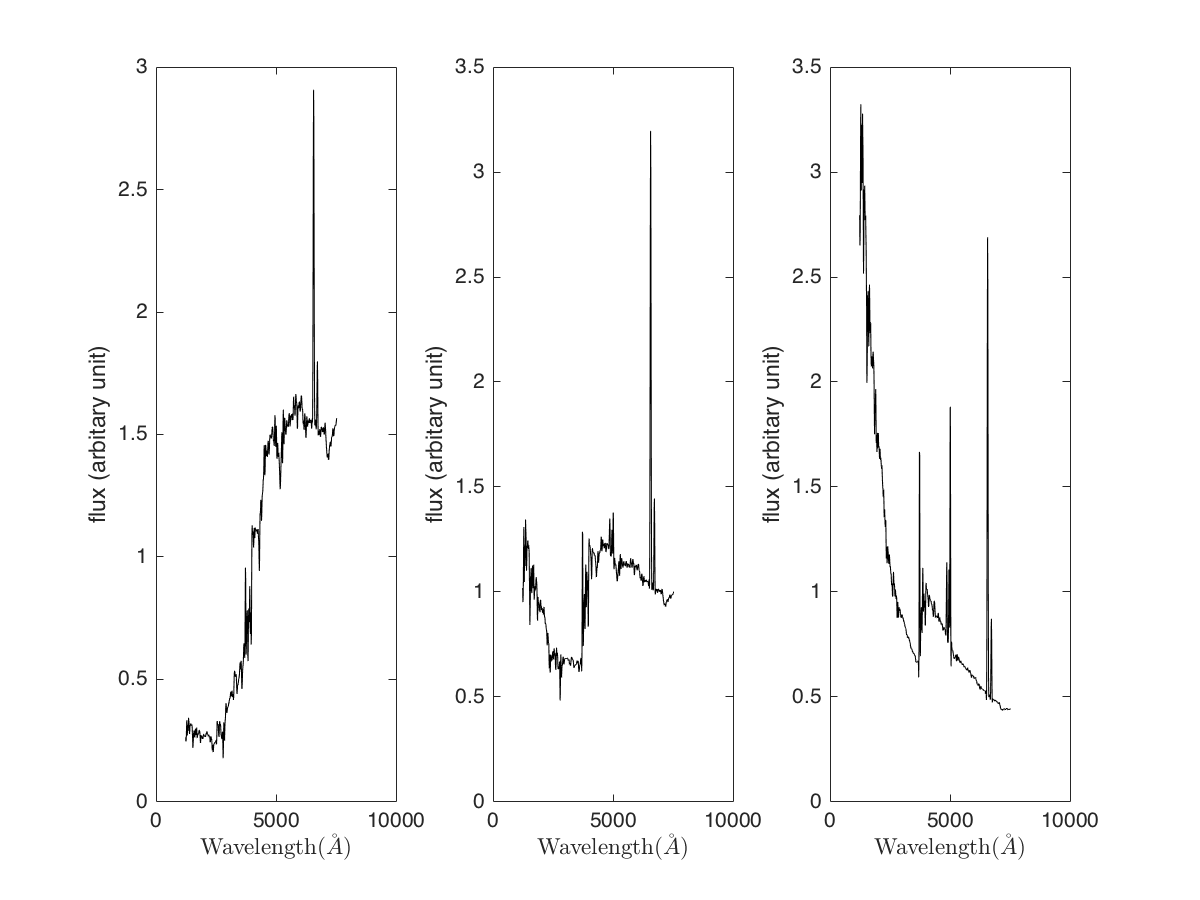
\includegraphics[width=\textwidth]{../images/1d/SED_total1by3.png}
                     %\caption{$1\times2$ hits map}
                     %\label{fig: 1by3Thits}
                \end{subfigure}
                \caption{Same as Fig.~\ref{fig: 1by2V}, but this time we used network with size of $1\times3$ to classify the sample galaxies.}
                \label{fig: 1by3V}
            \end{figure}       
            
            In Fig.~\ref{fig: 1by22V}, we used the $1\times22$~network to classify the the sample galaxies.
            As mentioned in the Sec.~\ref{sec: 1Dt}, this network size is the first size we could see, the K96 galaxies separated in 12 different neurons.
            B and E or SB1 and SB2 galaxies were too similar to SOM can recognize them as two separate groups.
            The same as Figs.~\ref{fig: 1by2V} and ~\ref{fig: 1by3V}, upper plot of the Fig.~\ref{fig: 1by22V} shows how many of galaxies from the 142 galaxies, moved to each neuron in the $1\times22$ SOM.
            \begin{figure*}
                \begin{subfigure}[b]{0.9\textwidth}
                    \centering
                    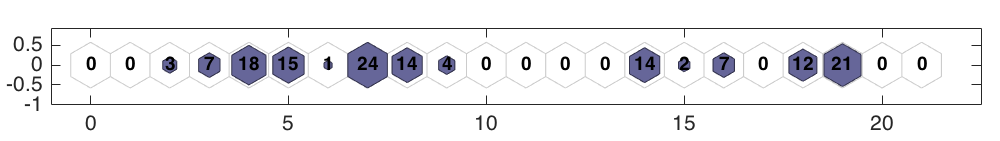
\includegraphics[width=\textwidth]{../images/1d/hit_v_1_by_22.png}
                    %\caption{$1\times2$ weight map}
                     %\label{fig: 1by3T}
                \end{subfigure}
                \hfill
                \begin{subfigure}[b]{0.9\textwidth}
                     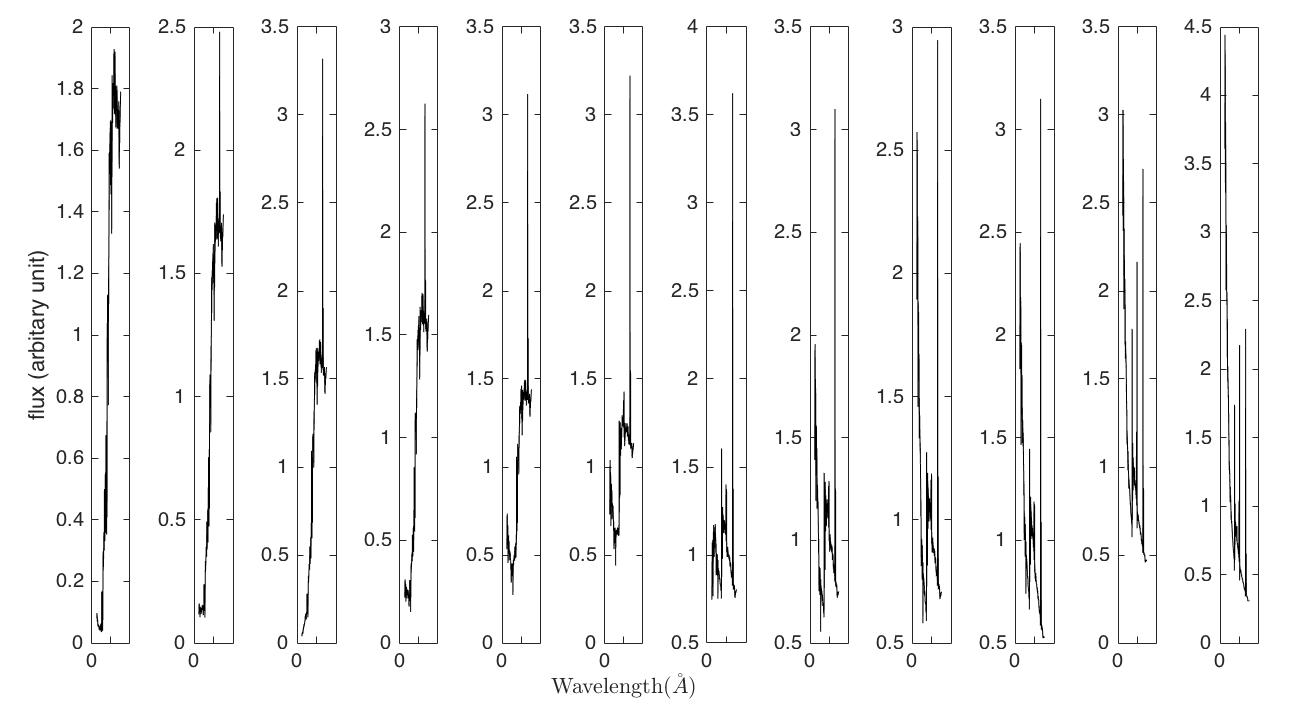
\includegraphics[width=\textwidth]{../images/1d/SED_total1by22.png}
                     %\caption{$1\times2$ hits map}
                     %\label{fig: 1by3Thits}
                \end{subfigure}
                \caption{Same as Fig.~\ref{fig: 1by2V}, but this time we used network with size of $1\times22$ to classify the sample galaxies.}
                \label{fig: 1by22V}
            \end{figure*}
            And the lower plot of the figure represents the average SED of the galaxies in each neurons.
            However, this time, since galaxies had more space to separated some of the neurons left empty. 
            Thus instead of having 22 average SED plots in the lower part of the Fig.~\ref{fig: 1by22V}, we have 12 SEDs.
            
            By comparing the upper part of Fig.~\ref{fig: 1by22V} with the lower part of the Fig.~\ref{fig: 1by22T}, we can see that the occupied neurons are not necessarily the same.
            If a groups of the T12 galaxies fills the same neurons as a K96 galaxies, we can conclude that this group of the galaxies have SEDs very similar to the SED of one of K96 galaxies.
            Whereas, we can conclude that a group of the galaxies have properties between the two groups if they fill a neuron which is empty and places between two categories of galaxies in the Fig.~\ref{fig: 1by22T}.
            However, the colours between these neurons in the upper side of the Fig.~\ref{fig: 1by22T}, establishes that the group of galaxies are more similar to which group.
            
            In the first two neurons of the upper plot in the Fig.~\ref{fig: 1by22V}, there is no galaxies, while in galaxies B and E are in the same neurons in the trained network.
            So we can conclude that there is no galaxies with similar
            There are 3 galaxies in the third neurons which shows these 3 galaxies are very much similar to the S0 type. 
            18 of the galaxies are on the fifth neurons and similar to the Sa type of the galaxies, while the 7 galaxies in the fourth neurons have SEDs similar to both S0 and Sa galaxies.
            There is one Sb type galaxy and 15 galaxies with SED similar to both Sa and Sb type galaxies.
            The following two neurons (eighth and ninth neurons from the left) are in the edge of the early type and star burst galaxies.
            In the upper plot in the  Fig.~\ref{fig: 1by22T}, the colour between these two neurons are black, which indicates that the weights between these two are really different from each other.
            Therefore, 24 galaxies in the eighth neurons have similar SEDs to Sb type galaxies and SEDs of the 14 galaxies in the ninth neurons are similar to the SB6 galaxies.
            The far right of the network, galaxies with SED comparable to type SB1 and SB2.
            
            In general from the 142 galaxies in T12, we categorized them as following; three of the galaxies belongs to SO galaxies, fifteen are Sa, one is Sb, four are SB6, two are SB5, and 21 have a similar SED to SB2.
            The rest of the galaxies have SEDs in between of the initial 12 suggestions.
            As T12 mentioned, part of the reason we could not classify all the galaxies using the K96 model is that the model were constructed from co-adding 12 spectra of the 70 galaxies.
            In this small sample, it is quite possible that the best SEDs do not match any model, perfectly and the original classifications have high uncertainty.
            
            On the other hand, all the other methods (i.e. $\chi^2$ fitting, trained neural network) of matching SEDs limit themselves to models, and if they could not find the best match, report the results as an uncertain ones.
            However, with SOM, galaxies have this freedom to be categorized in the intermediate groups.
            Therefore, if the SED of galaxies do not match completely with any of the model SEDs in Fig.~\ref{fig: k96}, they can be categorized as a SED with similarity to two or more of the groups.

                        
        \subsubsection{1D NETWORKS results and Properties of galaxies} 
    
    \subsection{2D SOMs}
    \label{sec: 2D}
    Although the 1D networks are great tools to categorize the SEDs and monitor the changes of properties of galaxies in each category, each neurons in these networks is limited to be connected to on other neurons in each direction.
    Since each neuron can have more than two immediate neighbours in the 2D networks, they provide more complete pictures of the relation between each SED type.
    For analysing 2D networks, we consider two approaches; at first we assumed that all the galac
    
    
    

    
    
    \subsection{Caveat}
    There is no established method to find the best SOM initial values. Size of the maps, number of neighbours in each steps, number of iterations could vary and each one give us a new result.
    Also, since at the beginning the weights are generated randomly, in each run the results could have small differences.
    
    